\chapter{La FIC}

\section{Cómo llegar}

La \textbf{\acrfull{FIC}} está ubicada en el \textbf{Campus de Elviña} de la \acrshort{UDC}. Su dirección es ``Camiño do Lagar de Castro, 6, 15008 A Coruña".

\subsection{Llegada en coche}

La \acrshort{FIC} cuenta con \textbf{espacio para aparcar junto a la facultad} y otros aparcamientos cercanos.

\FloatBarrier
\begin{figure}[htp]
    \centering
    \frame{\includegraphics[width=\linewidth]{figures/fic/como_llegar/FIC_parking.png}}
\end{figure}
\FloatBarrier

\subsection{Línea UDC}

La \acrshort{FIC} está situada cerca de tres paradas de la \textbf{línea de autobuses urbanos \acrshort{UDC}}: una en sentido entrante (\texttt{348 - Campus de Elviña, glorieta}) y dos en sentido saliente (\texttt{349 - Campus de Elviña, Informática} y \texttt{460 - Intercampus, glorieta Elviña}).

\FloatBarrier
\begin{figure}[htp]
    \centering
    \frame{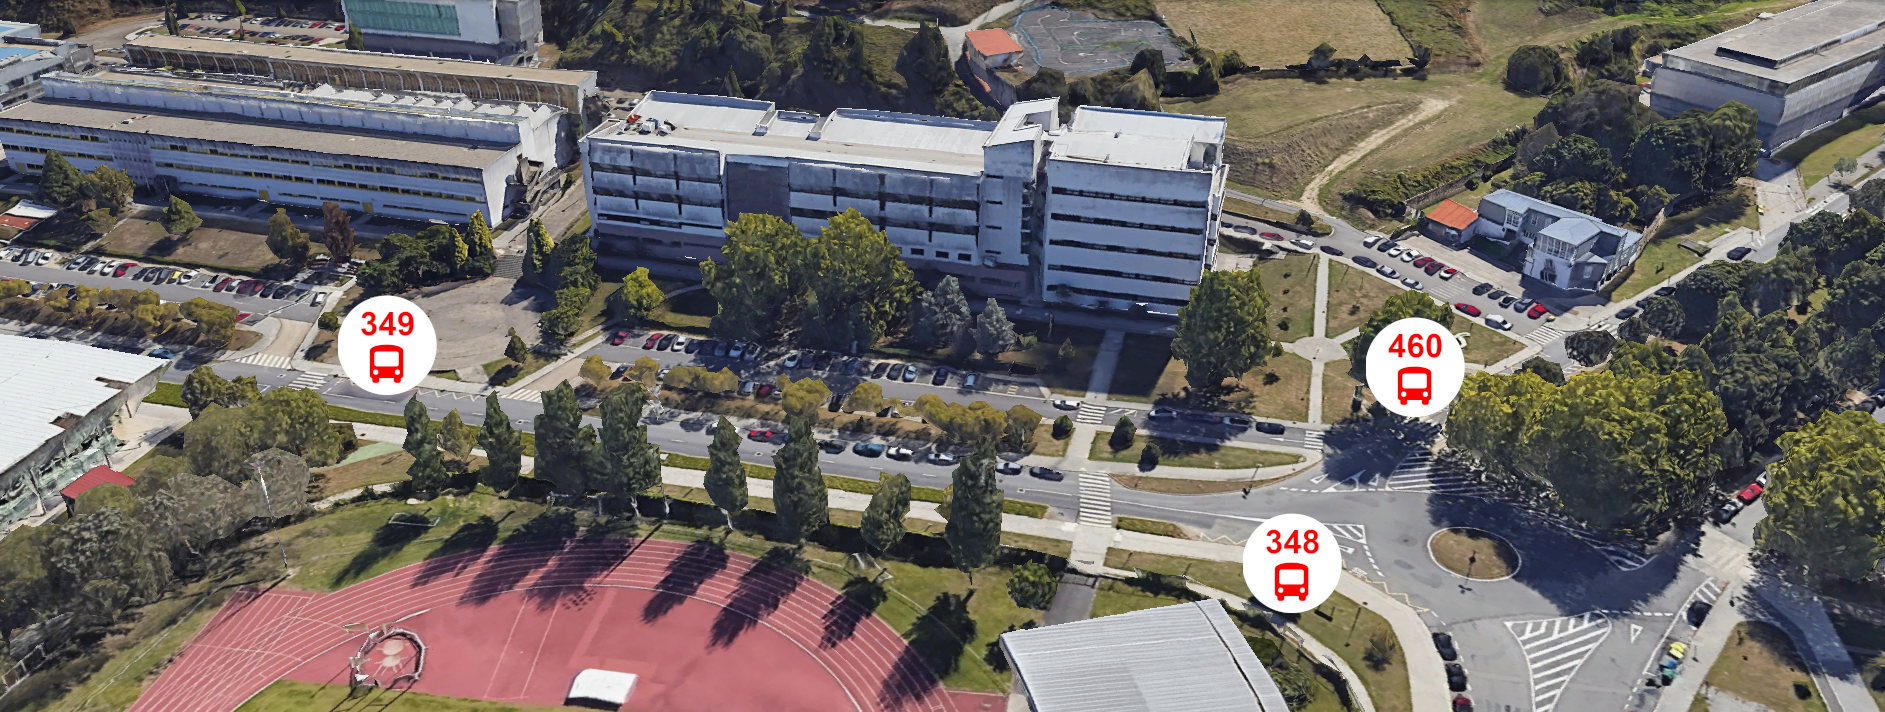
\includegraphics[width=\linewidth]{figures/fic/como_llegar/FIC_Buses.png}}
\end{figure}
\FloatBarrier

\begin{infoBox}
    Se puede consultar el tiempo estimado de llegada del autobús en la aplicación \href{https://tranviascoruna.com/}{\texttt{iTranvias}}.
\end{infoBox}


\section{Sitios web}

\subsection{Página Web de la FIC}

En  la \href{https://www.fic.udc.es/}{\textbf{página Web de la \acrshort{FIC}}} se muestran noticias, avisos importantes y ofertas de prácticas o empleo. También cuenta con varias secciones con información sobre la propia facultad, los estudios, servicios, premios, calendarios, horarios y más.

\FloatBarrier
\begin{figure}[htp]
    \centering
    \frame{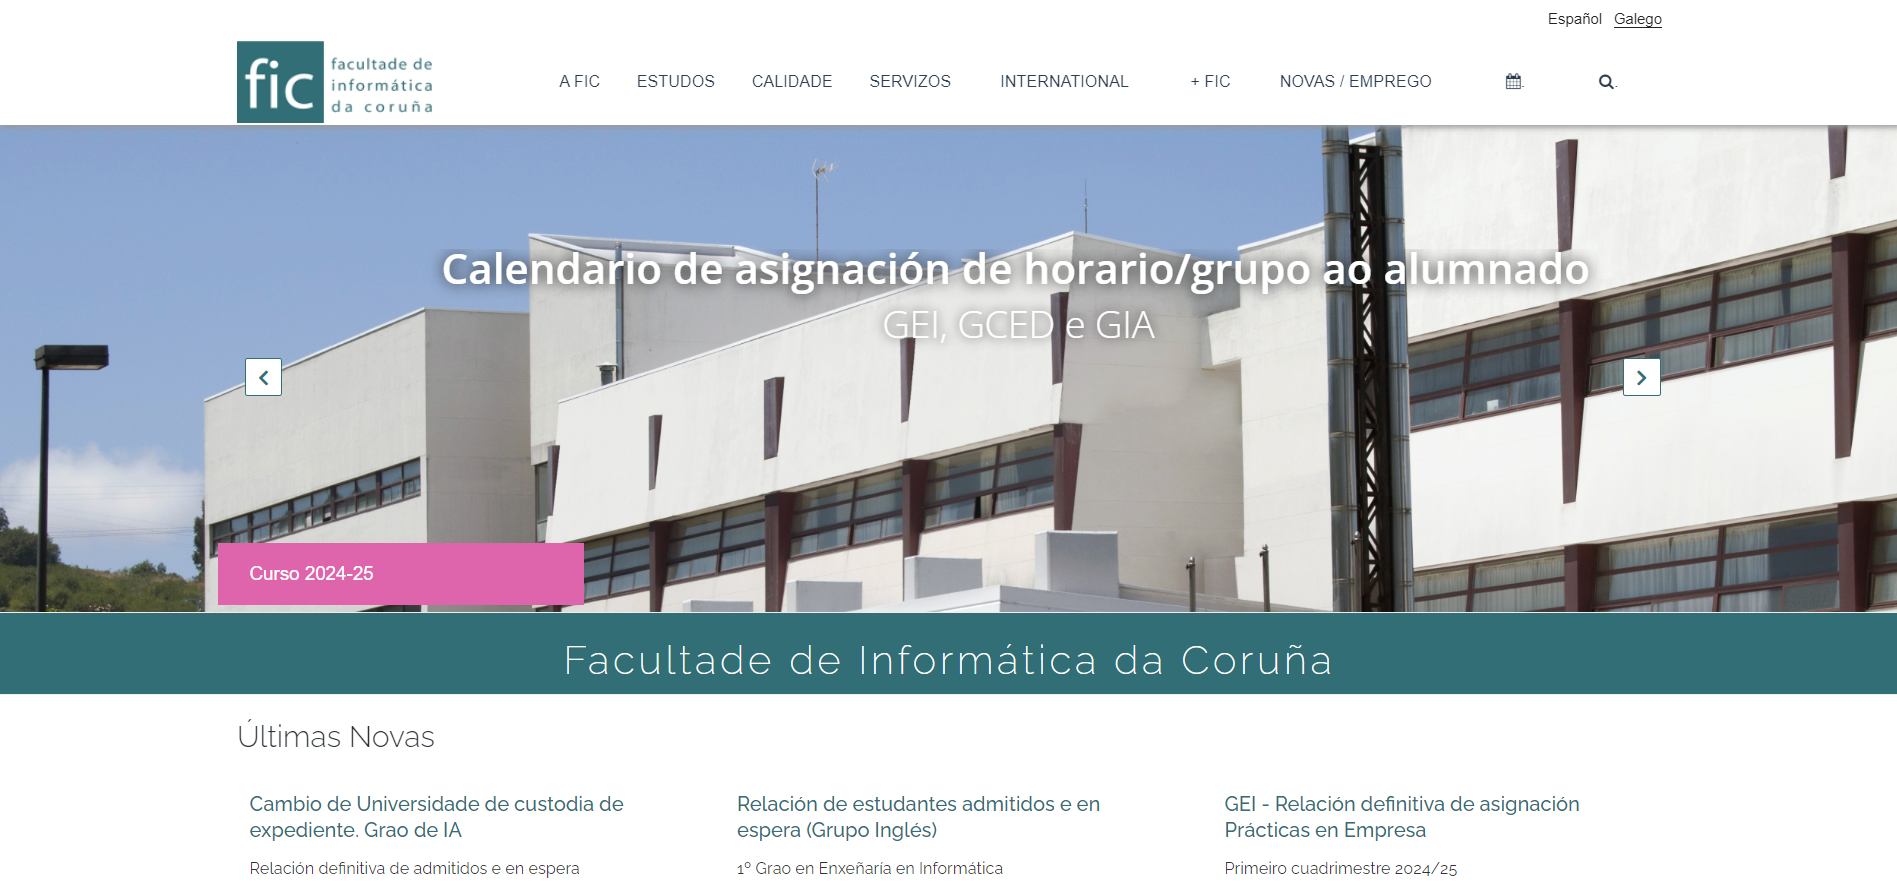
\includegraphics[width=\linewidth]{figures/fic/sitios_web/FIC_Web.png}}
\end{figure}
\FloatBarrier

\subsection{Tablón digital}

Los grados disponen de un \textbf{tablón digital} con información detallada sobre los plazos y procedimientos a seguir de las \textbf{prácticas en empresa} y \textbf{trabajos de fin de grado}.

\begin{infoBox}
    Cada estudio (\href{\linkTaboleiroGEI}{\acrshort{GEI}}, \href{\linkTaboleiroGCED}{\acrshort{GCED}}) tiene su propio tablón digital.
\end{infoBox}

\begin{warningBox}
    El acceso a cada tablón digital está \textbf{restringido} al alumnado del mismo estudio.
\end{warningBox}

\subsection{Redes sociales}

La \acrshort{FIC} publica \textbf{información de interés} en su canal de \href{https://t.me/+LHa3QApmGskyNDFk}{\faIcon{telegram}~\textbf{Telegram}} y en su cuenta de \href{https://x.com/FIC_UDC}{\faIcon{twitter}~\textbf{Twitter/X}} (@FIC\_UDC).

También sube \textbf{contenido} ocasional a su canal de \href{https://www.youtube.com/@facultaddeinformaticadeaco4211}{\faIcon{youtube}~\textbf{YouTube}} como eventos o transmisiones de las ceremonias de graduación.


\section{Espacios}

La \acrshort{FIC} cuenta con \textbf{5 plantas} (0, 1, 2, 3 y 4) que comprenden varias aulas, despachos, laboratorios, salas especiales y espacios de servicios.

\begin{infoBox}
    Algunos espacios cuentan con \textbf{identificadores} con una \textbf{letra} que indica el \textbf{tipo de espacio} (`A' para aula, `L' para laboratorio, `S' para seminario...) y un \textbf{primer número} que indica la \textbf{planta} en la que están ubicados.
\end{infoBox}

\subsection{Aulas y laboratorios de prácticas}

\subsubsection{Aulas}

Las \textbf{aulas} están ubicadas las plantas 2 y 3 de la 
\acrshort{FIC}. Estas aulas son en las que se imparten las \textbf{clases teóricas} y algunas clases de prácticas. Existen cuatro aulas grandes (con 120 plazas) y otras de menor tamaño. Todas cuentan con proyector y equipo informático para el profesor.

\subsubsection{Laboratorios de prácticas}

Existen varios \textbf{laboratorios} para la realización de las \textbf{prácticas}, incluyendo un laboratorio de electrónica y robótica (L0.6). Estos laboratorios están situados en las plantas 0 y 1.

\subsection{Despachos, seminarios y laboratorios de investigación}

\subsubsection{Despachos}

En los \textbf{despachos} puede encontrarse al profesorado para ser consultado o realizar tutorías. Hay despachos en  todas las plantas de la \acrshort{FIC}.

\begin{infoBox}
    Algunos profesores tienen sus despachos en otras facultades o en el Área Científica.
\end{infoBox}

\subsubsection{Seminarios}

Los \textbf{seminarios} cuentan con espacios adaptados a la realización de otras actividades como celebración de reuniones, impartición de cursos o videoconferencias.

\subsubsection{Laboratorios de investigación}

Son \textbf{laboratorios} donde desarrollan sus trabajos de \textbf{investigación} el personal docente del centro, los doctorandos en fase de elaboración de tesis y los contratados para proyectos de investigación subvencionados. Están ubicados en todas las plantas de la \acrshort{FIC}.

\subsection{Espacios de servicios}

\subsubsection{Conserjería}

La \textbf{conserjería} está en la planta 1 de la \acrshort{FIC}. Su personal es el que se encarga de la apertura y cierre del centro y del correcto mantenimiento de todos sus servicios e instalaciones. Los objetos perdidos (y encontrados) también pueden dejarse aquí.

\textbf{Horario}: De 08:15 (15 minutos después de la apertura del centro) a 21:30, de lunes a viernes.

\begin{curiosityBox}
    Junto a consejería hay un \textbf{buzón rojo} en el que se pueden depositar quejas, sugerencias y felicitaciones.
\end{curiosityBox}

\subsubsection{Administración y secretaría}

La \textbf{secretaría} de la \acrshort{FIC} está situada en la planta 1. Es el lugar en que se realizan los \textbf{trámites}.

\textbf{Horario}: De 08:30 a 14:00, de lunes a viernes.

\begin{warningBox}
    Para la mayoría de los trámites se requiere contar con  \href{https://outlook.office365.com/book/UNIVERSIDADEDACORUA8@udcgal.onmicrosoft.com/}{\textbf{cita previa}}.
\end{warningBox}

\begin{infoBox}
    Pueden consultarse los \textbf{horarios} de verano y festivos en la \href{https://www.fic.udc.es/gl/horario}{página web de la \acrshort{FIC}}.
\end{infoBox}

\subsubsection{Biblioteca}

La \textbf{biblioteca} de la \acrshort{FIC} se encuentra en la planta 1. Cuenta con una colección de aproximadamente 25.570 ejemplares que cubren las diversas áreas del conocimiento de la \acrshort{FIC} en la que destaca una sección de títulos recomendados entre los que se encuentran las lecturas básicas de las asignaturas impartidas. También es posible consultar \textbf{revistas}, \textbf{memorias de \acrlong{TFG}} y \textbf{tesis doctorales}.

\textbf{Horario}: De 08:30 a 21:30, de lunes a viernes.

\textbf{Sitio web}: \url{https://www.udc.gal/biblioteca.fic/}

\begin{infoBox}
    Pueden consultarse los \textbf{horarios} de verano y festivos en la \href{https://www.fic.udc.es/gl/biblioteca-0}{página web de la \acrshort{FIC}}.
\end{infoBox}

\begin{curiosityBox}
    Junto a la biblioteca hay un \textbf{punto de recogida de libros} descatalogados.
\end{curiosityBox}

\begin{rememberBox}
    Pueden realizarse \textbf{préstamos} de libros con la \textbf{\acrshort{TUI}}. 
\end{rememberBox}

\subsubsection{Cafetería}

La \textbf{cafetería} está ubicada en la planta 1. Ofrece servicio de bebidas y comidas, incluyendo menú del día (el cual es publicado en \href{https://t.me/CafeteriaFIC}{\faIcon{telegram}~\textbf{Telegram}}) por 7.30\euro~ (precio de estudiante).

\textbf{Horario}: De 08:00 a 19:00, de lunes a viernes.

\textbf{Carta}: \url{https://quecarta.com/cafeteria-fic-}

\begin{curiosityBox}
    En la cafetería de la \acrshort{FIC} existe una \textbf{opción vegana}.
\end{curiosityBox}

\subsection{Otros espacios destacados}

\subsubsection{Planta 0}

\begin{itemize}
    \item \textbf{Zona de mesas}: Existen varias mesas con tomas eléctricas y sillas donde el alumnado puede trabajar o pasar el tiempo entre clases.

    \item \textbf{Salón de Actos}: En este se realizan grandes eventos como la jornada de bienvenida a la \acrshort{FIC} para los estudiantes de primer curso, la presentación de empresas en la Feria de Empleo de la Facultad de Informática (\acrshort{FEPE}), entregas de premios como los premios a mejor \acrlong{TFG} de la \acrshort{FIC} o la ceremonia de graduación. Tiene capacidad para 520 personas.
\end{itemize}

\subsubsection{Planta 1}

\begin{itemize}

    \item \textbf{Decanato}: Se encuentra junto a la conserjería y en frente de la cafetería. 

    \item \textbf{Taquillas}: Están situadas en frente de la biblioteca. Funcionan con llave y cierre de moneda de 1\euro~ o 50 céntimos.
    
\end{itemize}

\subsubsection{Planta 2}

\begin{itemize}
    \item \textbf{Aula de Grados}: El aula de grados se utiliza principalmente para eventos tales como defensas de \acrshort{TFG} y de tesis doctorales. También se han organizado charlas para el alumnado en ella. Cuenta con capacidad para 45 personas. 
\end{itemize}

\begin{curiosityBox}
    Este aula es denominada oficialmente como “Aula de Graos Víctor Gulías”. Debe su nombre a \href{https://badalnovas.com/2024/01/28/in-memoriam-victor-manuel-gulias-fernandez-10o-aniversario-do-seu-falecemento/}{Víctor Manuel Gulías Fernández}, fallecido en 2012. Por aquel entonces, era director del \acrshort{CITIC}, profesor titular de la \acrshort{FIC} y vicedecano para la relación con la Industria.   
\end{curiosityBox}

\subsubsection{Planta 3}

\begin{itemize}
    \item \textbf{Local de alumnos}: Es donde se reúnen los \href{https://www.fic.udc.es/gl/delegacion-e-asociacions}{\textbf{representantes de estudiantes}}.
\end{itemize}
